Muchas sociedades en está última década han estado esforzándose por dejar de depender de combustibles
fósiles y sus derivados debido a potenciales riesgos geopolíticos, económicos y ambientales. La energía solar
es una de las fuentes de energía alternativas de mayor interés por su fácil acceso y casi ilimitado suministro.
Sin embargo, el aprovechamiento de esta energía requiere de dispositivos que deben ser capáces de capturar, transformar 
y almacenar la mayor cantidad de energía lumínica en trabajo útil en rangos de tiempo variantes a causa del tiempo atmosférico y
los estadíos solares.

\begin{figure}[h]
    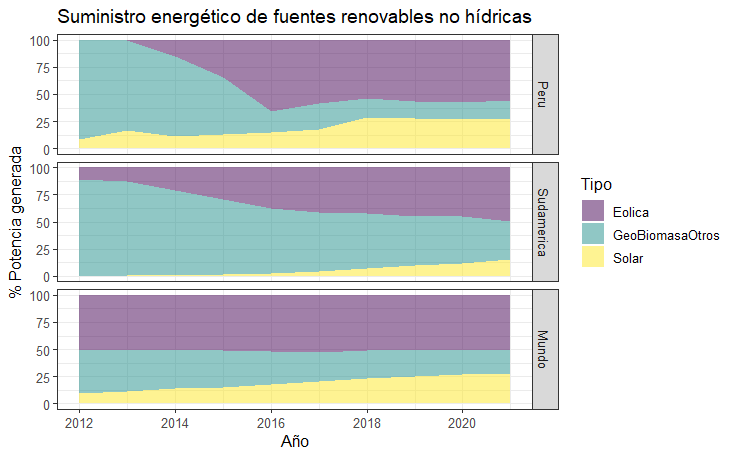
\includegraphics[scale=0.8]{img/PorcentajeRenovables.png}
\end{figure}

La tecnología termosolar condensa el haz solar en un contenedor de un fluído de tal manera que este se caliente
y mueva un alternador eléctrico, mientras que la energía fotovoltaica convierte la radiación solar en energía electroquímica directamente 
por medio de fenómenos fotovoltaicos que se accionan gracias a materiales rececptores, transformadores y transportadores de carga.
Las centrales termosolares tienen el potencial de generar miles de kilos-vatios por hora (KWh) no obstante 
existen desventajas que limitan la difusión de su uso tales como su alto costo en la instalación, mantenimiento y distribución por cableado 
eléctrico, así como la gran cantidad de energía desperdiciada en los procesos de transferencia de calor. Estos problemas están casi ausentes
en los sistemas fotovoltaicos ya que se usan paneles y modulos que facilitan su uso, sin embargo aún es un reto equiparar la eficiencia de estos 
dispositivos con los termosolares. Si bien existen tecnologías que unen la termosolar y fotovoltaica, el presente trabajo se enfoca en resolver
un problema dentro de la fotovoltaica.

Los sistemas fotovoltaicos llevan en el mercado cerca de 60 años, desde su \hl{lanzamiento por Laboratorios Bell en 1963}. El corazón funcional de estos 
dispositivos son las celdas solares, las cuales consisten en placas compuestas por láminas superpuestas de materiales que pueden transportar carga 
entre electrodos gracias al cambio de potencial que sufren en presencia de radiación solar. La basta variedad de materiales que han sido empleados para 
otorgarle propiedades fotoactivas, también conocidos como sensibilizantes, hace difícil clasificarlos según su naturaleza, por eso Rathore y su equipo 
se basaron en la antigûedad comercial para categorizar las celdas en tres generaciones \cite{rathore2021}. La primera generación consiste en celdas 




\begin{itemize}
    \item Cerca del \%80 de la población mundial viven de las importaciones 
     de combustibles fósiles son vulnerables a sufrir crisis energéticas
     debido a problemas geopolíticas y económicas.
     (IRENA)
    
    \item Las fuentes de energías 
\end{itemize}
